%%%%%%%%%%%%%%%%%%%%%%%%%%%%%%%%
%Norme di Progetto main file
%Version:0.0.1
%Author:Alberto Adami(alberto.adami.7@gmail.com)
%Creation Date:2013-12-07
%%%%%%%%%%%%%%%%%%%%%%%%%%%%%%%%%
\section{Protocollo per la gestione del progetto}
\label{protocollo}
Il servizio GitHub\glossario{}, al suo interno incorpora un sistema per la gestione dei ticket e creazione di milestone\glossario{}. Si è quindi deciso di usufruire di tali servizi.
\subsection{Creazione milestone}
\label{milestone}
Il \projectManager{} dovrà provvedere alla creazione di una milestone\glossario{} per la prossima revisione a cui il gruppo \authorName{} ha intenzione di partecipare.
\\Per creare una nuova milestone\glossario{} bisogna:
\begin{itemize}
\item Cliccare su issue;
\item Andare su milestone\glossario{};
\item Premere su \lq\lq{}Create a new milestone\glossario{}\rq\rq{};
\item Infine vanno compilati i campi richiesti\footnote{I possibili cambi da completare sono riportati in Figura \ref{github_milestone}.}.
\end{itemize}
Si potrà vedere lo stato di avanzamento della milestone\glossario{} guardando il numero di ticket completati rispetto ai ticket totali.
\begin{figure}[h]
	\centering
	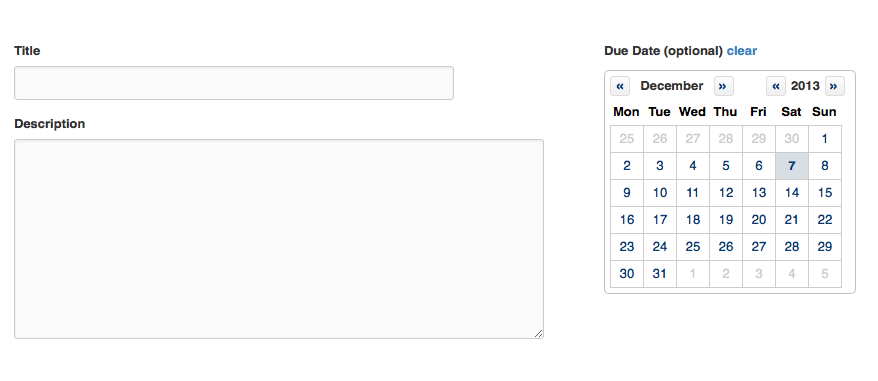
\includegraphics[width=15cm]{./content/Immagini/Screen1.png}
	\caption{Interfaccia di GitHub per la creazione di una milestone}
	\label{github_milestone}
\end{figure}
\pagebreak
\begin{figure}[!h]
	\centering
	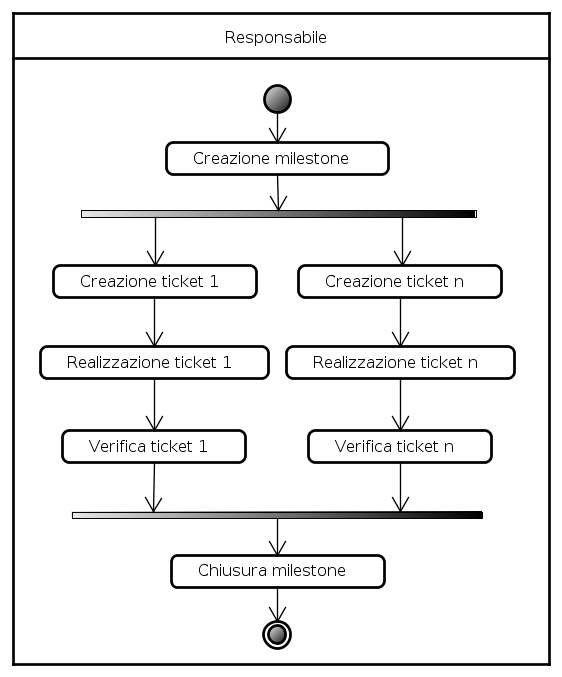
\includegraphics[height=8cm]{./content/Immagini/Avanzamento_Milestone.png}
	\caption{Modello per la gestione di una milestone}
	\label{gestione_milestone}
\end{figure}
\subsection{Creazione ticket}
\label{cticket}
I ticket vengono creati da:
\begin{itemize}
\item \textbf{\projectManager:} crea la maggioranza dei ticket;
\item \textbf{\emph{Verificatore}:} crea i ticket per segnalare le imprecisioni o errori trovati durante la verifica.
\end{itemize}
Ogni ticket dovrà essere assegnato ad un unico membro del team \authorName{} e dovrà avere le seguenti caratteristiche\footnote{In figura 3 è mostrata l'interfaccia per la creazione di ticket.}:
\begin{itemize}
\item{\textbf{Destinatario:}} a chi è rivolto l'attività indicata dal ticket;
\item{\textbf{Milestone:}} la milestone\glossario{} a cui è associato il ticket;
\item{\textbf{File:}} dovrà essere indicato il file oggetto dell'attività;
\item{\textbf{Label:}} ogni ticket avrà una o più label associate; le label possibili sono le seguenti:
\begin{itemize}
\item\textbf{Modifica:} ticket generalmente creato dal \emph{Verificatore} per segnalare gli errori trovati;
\item\textbf{Verifica:} ticket creato dal \projectManager{} per assegnare la verifica a uno dei \emph{Verificatori};
\item\textbf{Richiesta approvazione:} ticket creato da un \emph{Verificatore} per richiedere l'approvazione di un documento;
\item\textbf{Creazione:} ticket creato dal \projectManager{} per assegnare un compito a un generico membro del gruppo;
\item\textbf{Priorità alta:} label assegnata ad un ticket creato per la gestione di anomalie;
\item\textbf{Priorità media:} label assegnata ad un ticket creato per la gestione di discrepanze di media gravità;
\item\textbf{Priorità bassa:} label assegnata ad un ticket creato per la gestione di discrepanze non gravi.
\end{itemize}
\end{itemize}
\begin{figure}[h!]
	\centering
	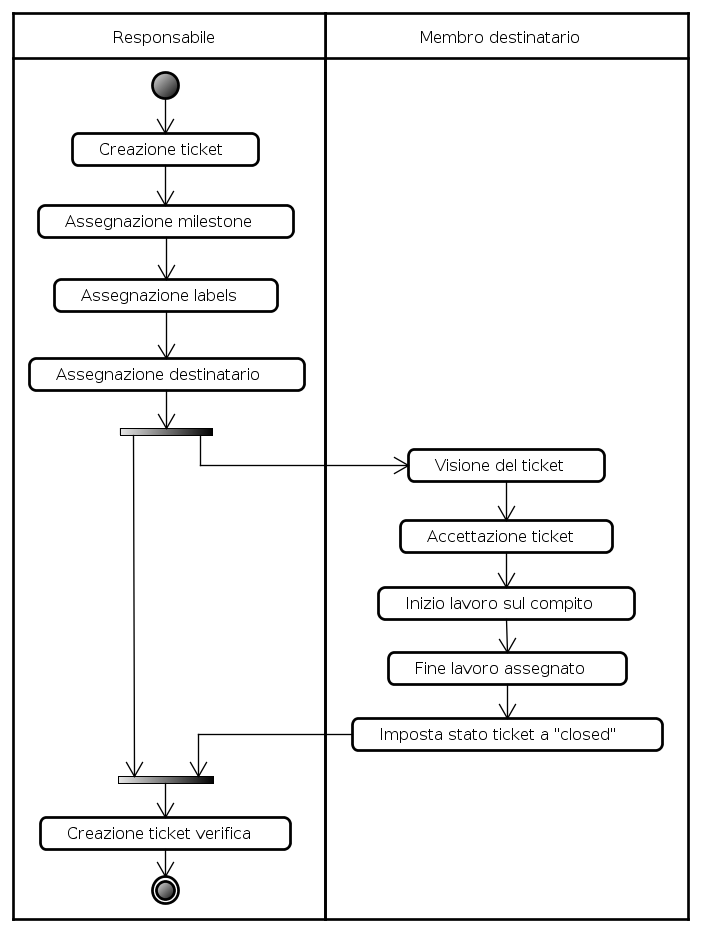
\includegraphics[height=10cm]{./content/Immagini/Creazione_Compito.png}
	\caption{Modello di ticket per la creazione di un compito generico}
	\label{creazione_ticketstd}
\end{figure}
\pagebreak
\begin{figure}[h!]
	\centering
	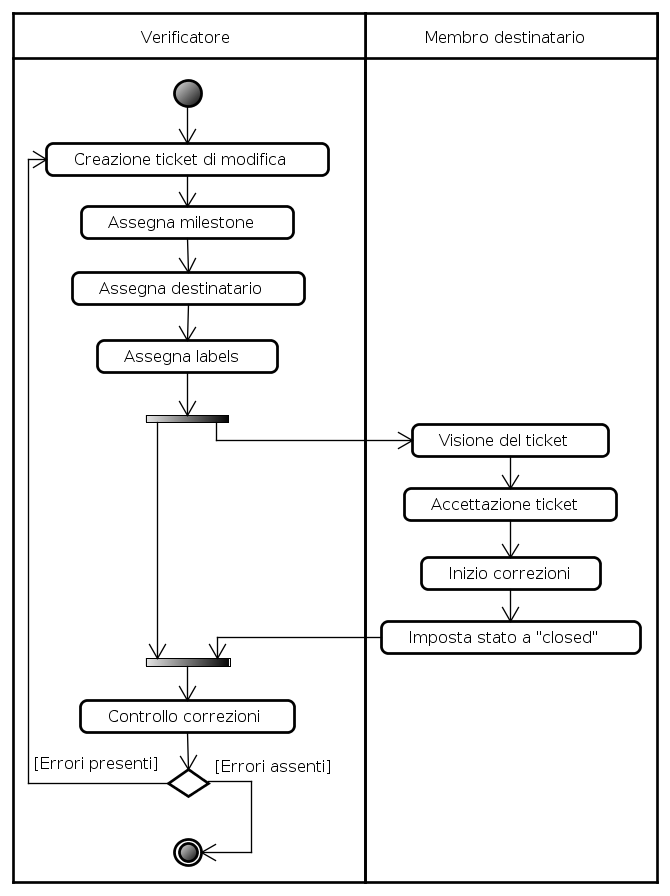
\includegraphics[height=10cm]{./content/Immagini/Ticket_Verificato.png}
	\caption{Modello di ticket per la creazione di un ticket di verifica}
	\label{creazione_ticketver}
\end{figure}
\pagebreak
\subsection{Esecuzione dei compiti}
\label{esecuzionecompiti}
\begin{figure}[h!]
	\centering
	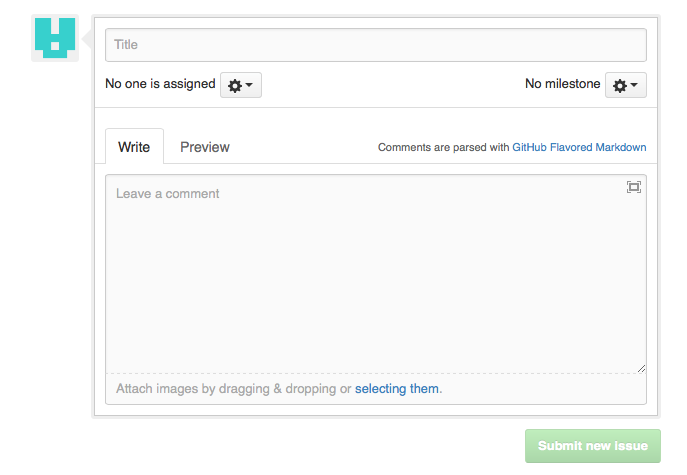
\includegraphics[width=12cm]{./content/Immagini/Screen2.png}
	\caption{Interfaccia di GitHub per la creazione di un ticket.}
\end{figure}
Ogni membro del gruppo dovrà visionare i ticket a lui assegnati e, successivamente all'esecuzione del compito, dovrà cambiare lo stato del ticket in \lq\lq{}closed\rq\rq{}.
\\Quando il destinatario del ticket ne prenderà visione, dovrà confermarlo con un commento nella pagina web del ticket. 
\\Se il \projectManager{} si rende conto che un ticket non è stato eseguito come atteso, \lq\lq{}riaprirà\rq\rq{} il ticket.
\subsection{Chiusura della milestone}
\label{chiusura}
Una volta raggiunta la scadenza o terminati tutti i ticket, la milestone\glossario{} verrà chiusa.
\\Successivamente il \projectManager{} provvederà alla creazione di una nuova milestone\glossario{} e tutto il protocollo ricomincerà da capo.
